%
\documentclass[10pt,a4paper]{article}


\usepackage{array}
\usepackage{subfigure}
\usepackage{graphicx}
\usepackage{amssymb}
\usepackage{amsmath}
\usepackage{cite}
\usepackage{color}
\usepackage{url}
\usepackage[lined,linesnumbered,ruled,norelsize]{algorithm2e}
\usepackage{listings}
\lstset{
  language=Octave, 
  basicstyle=\footnotesize, 
  frame=single, 
  showspaces=false, 
  showstringspaces=false}
\date{}




\begin{document}

\title{Technical Report 4: Regularization}

\maketitle

\section{Normal Equations for Linear Regression}
%
  The 5-order linear regression results with different regularization parameters are illustrated in Fig.~\ref{fig:data}. It can be observed that, the boundary well separates the positive data samples from the negative ones. As shown in Fig.~\ref{fig:data} (a), when $\lambda=0$, the regularization is disabled, such that the resulting curve perfectly fits the given data points. In this overfitting case, the regression results actually cannot show a general trend and thus may not be able to make an accurate prediction. By tuning $\lambda$, we have more control over the data fitting. In Fig.~\ref{fig:data} (b), we have a ``simplified'' fitting curve under $\lambda=1$. The curve does not fit the training data perfectly, but still demonstrate the trend of the data. In Fig.~\ref{fig:data} (c) where $\lambda=10$, the curve is too ``smooth'' to fit the training data. This case is so-called ``underfitting''.
  %
%
    \begin{figure}[htb!]
       \begin{center}
       \parbox{.32\columnwidth}{\center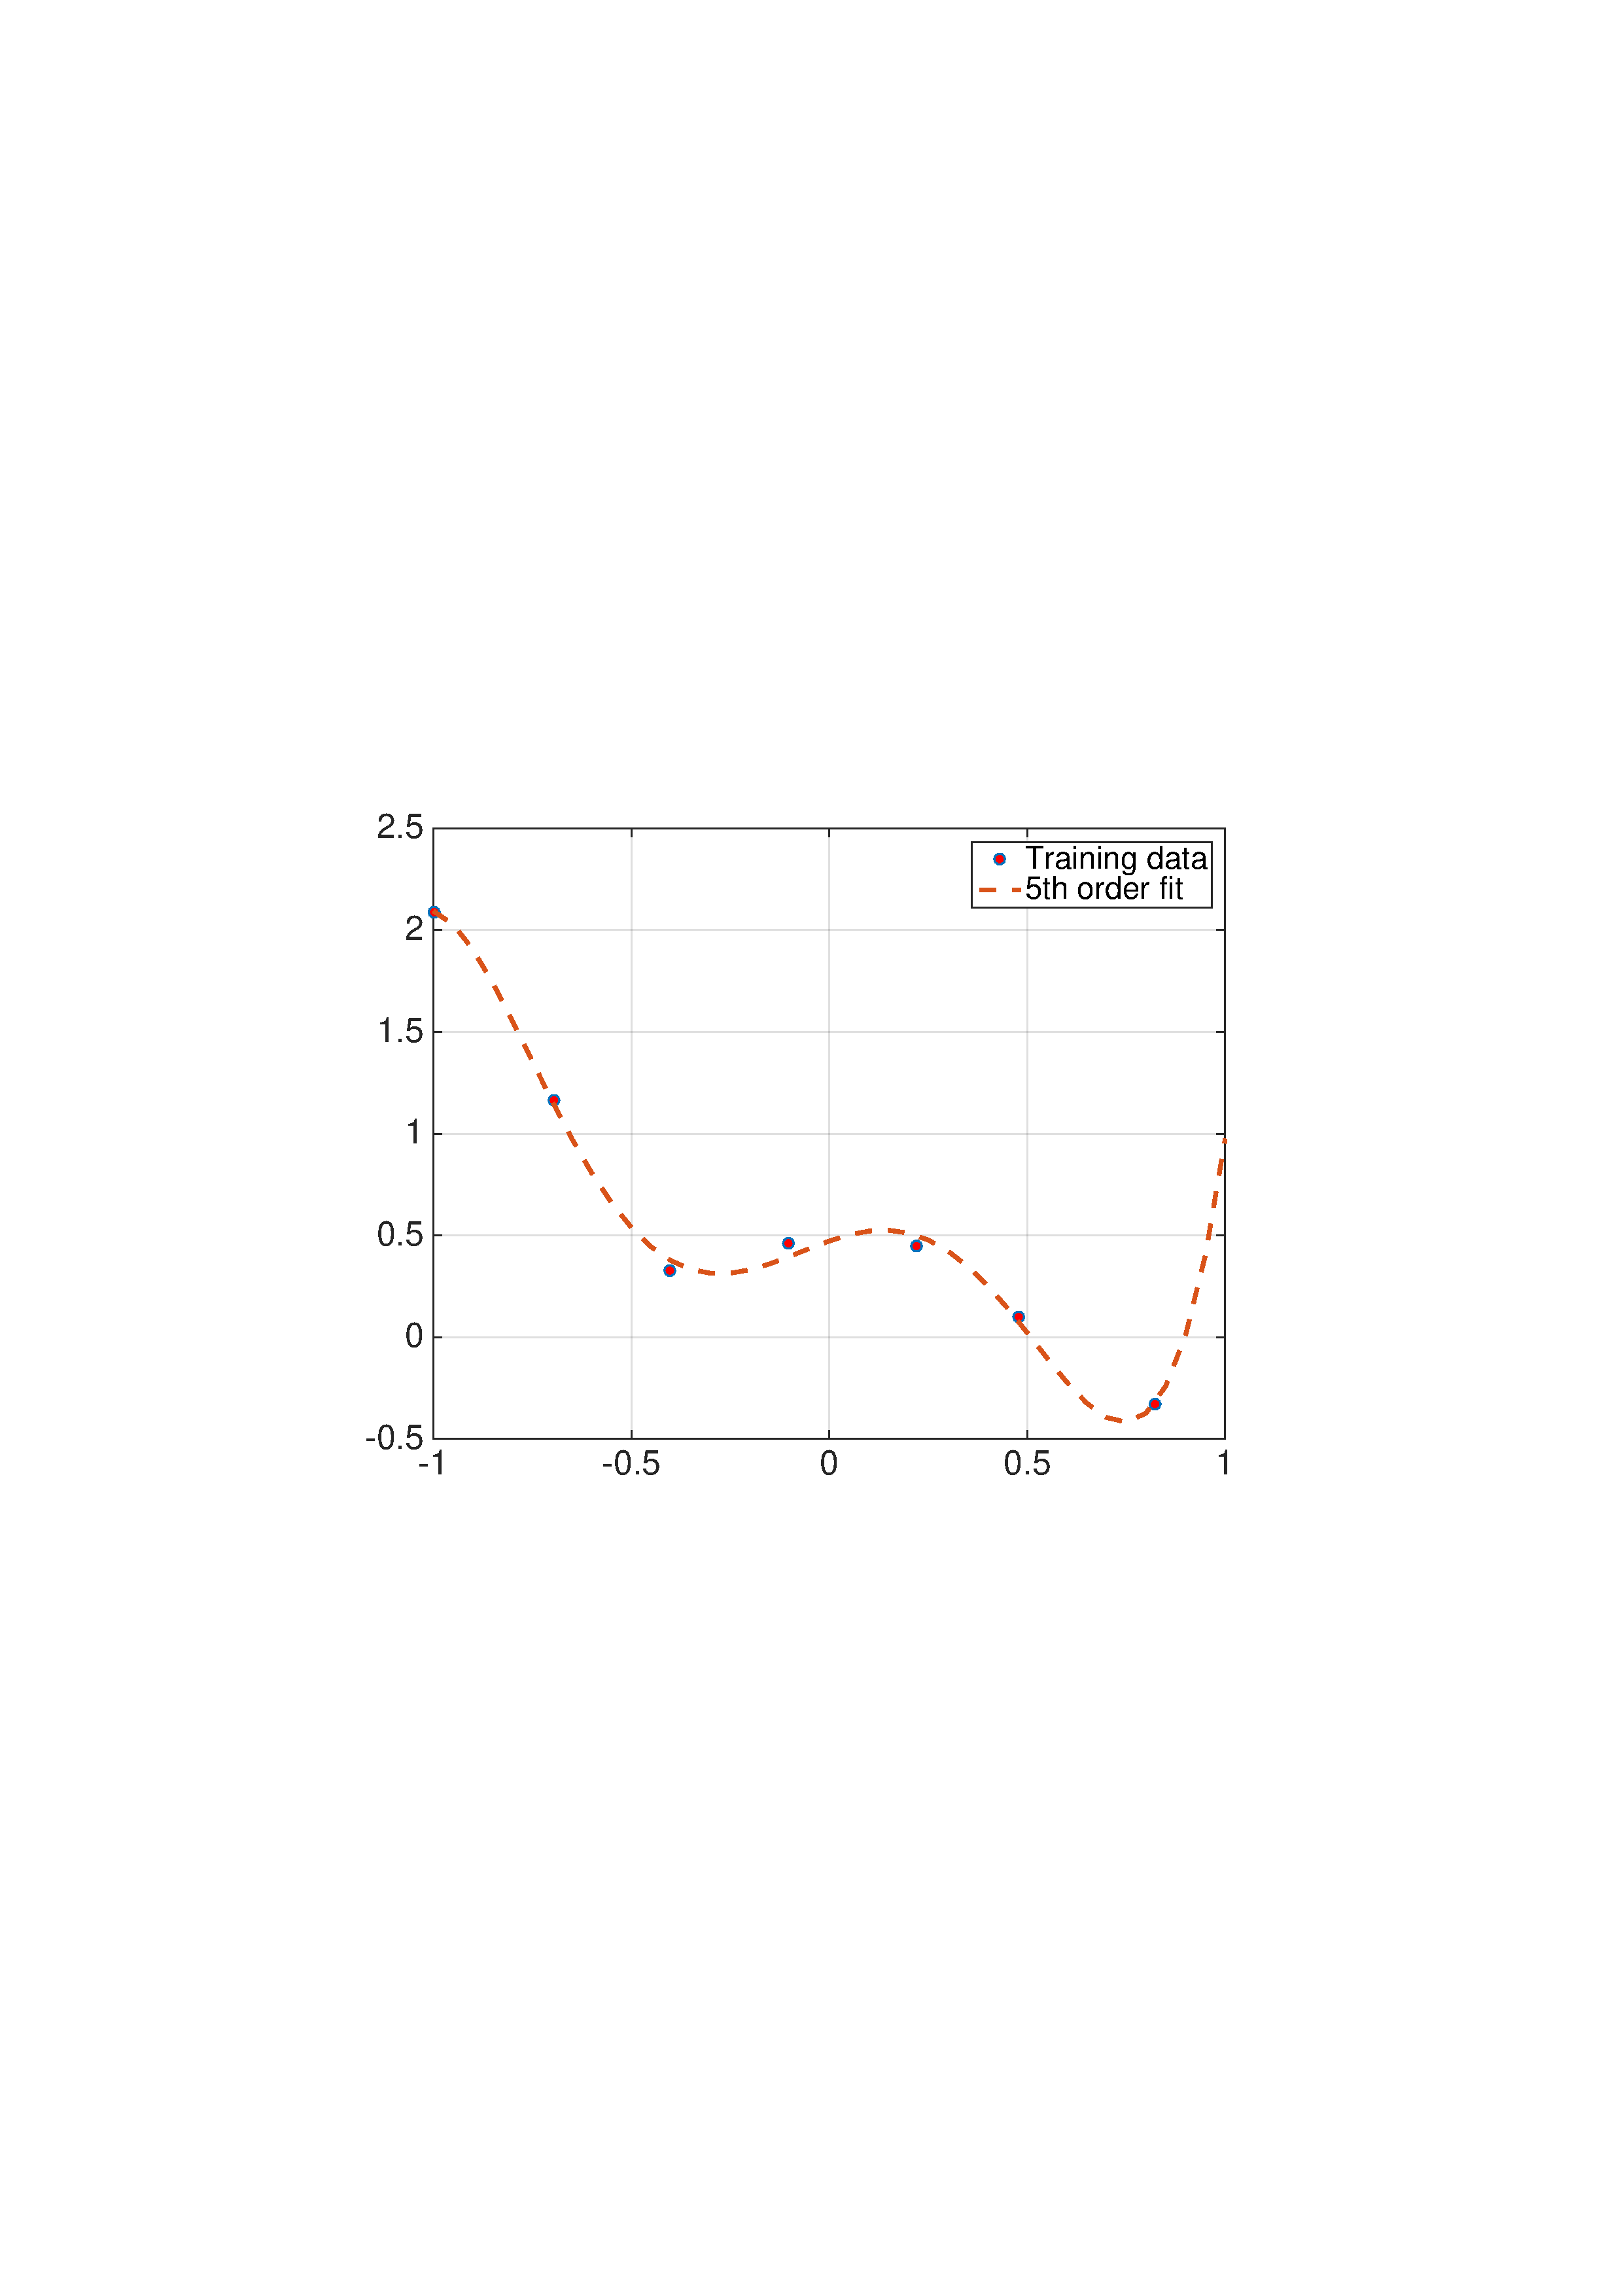
\includegraphics[width=.32\columnwidth]{lambda0}}
       \parbox{.32\columnwidth}{\center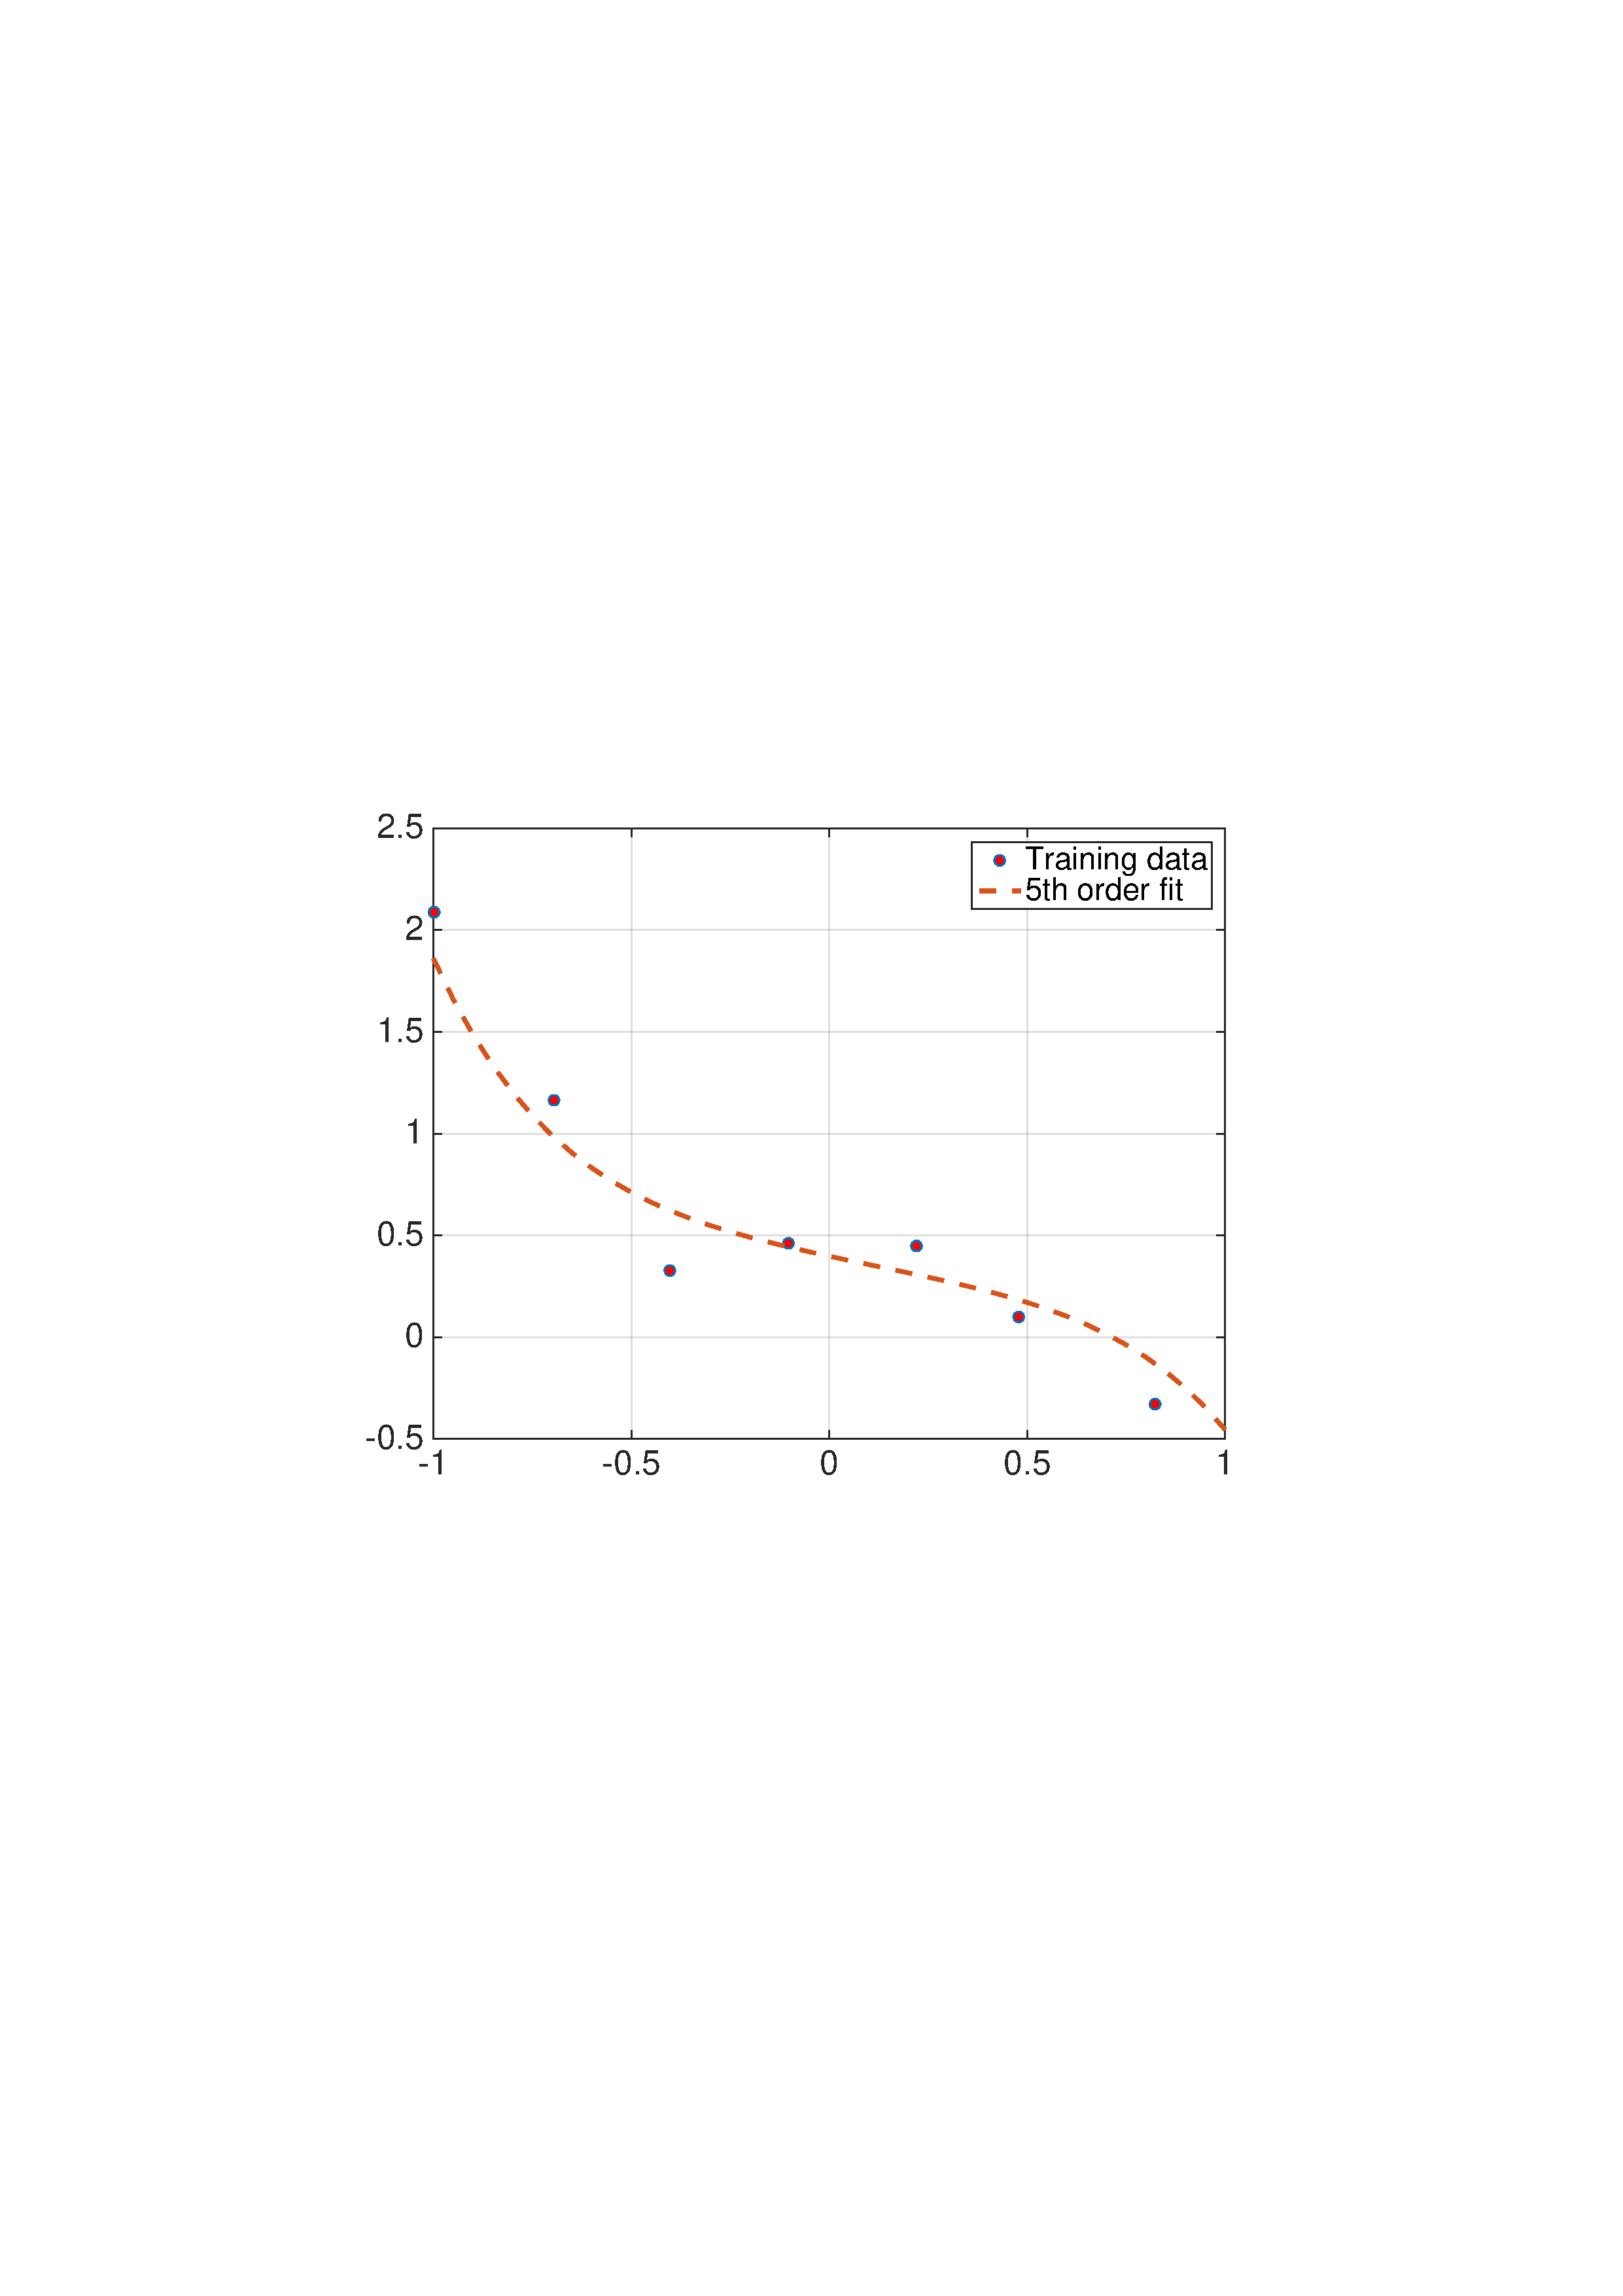
\includegraphics[width=.32\columnwidth]{lambda1}}
       \parbox{.32\columnwidth}{\center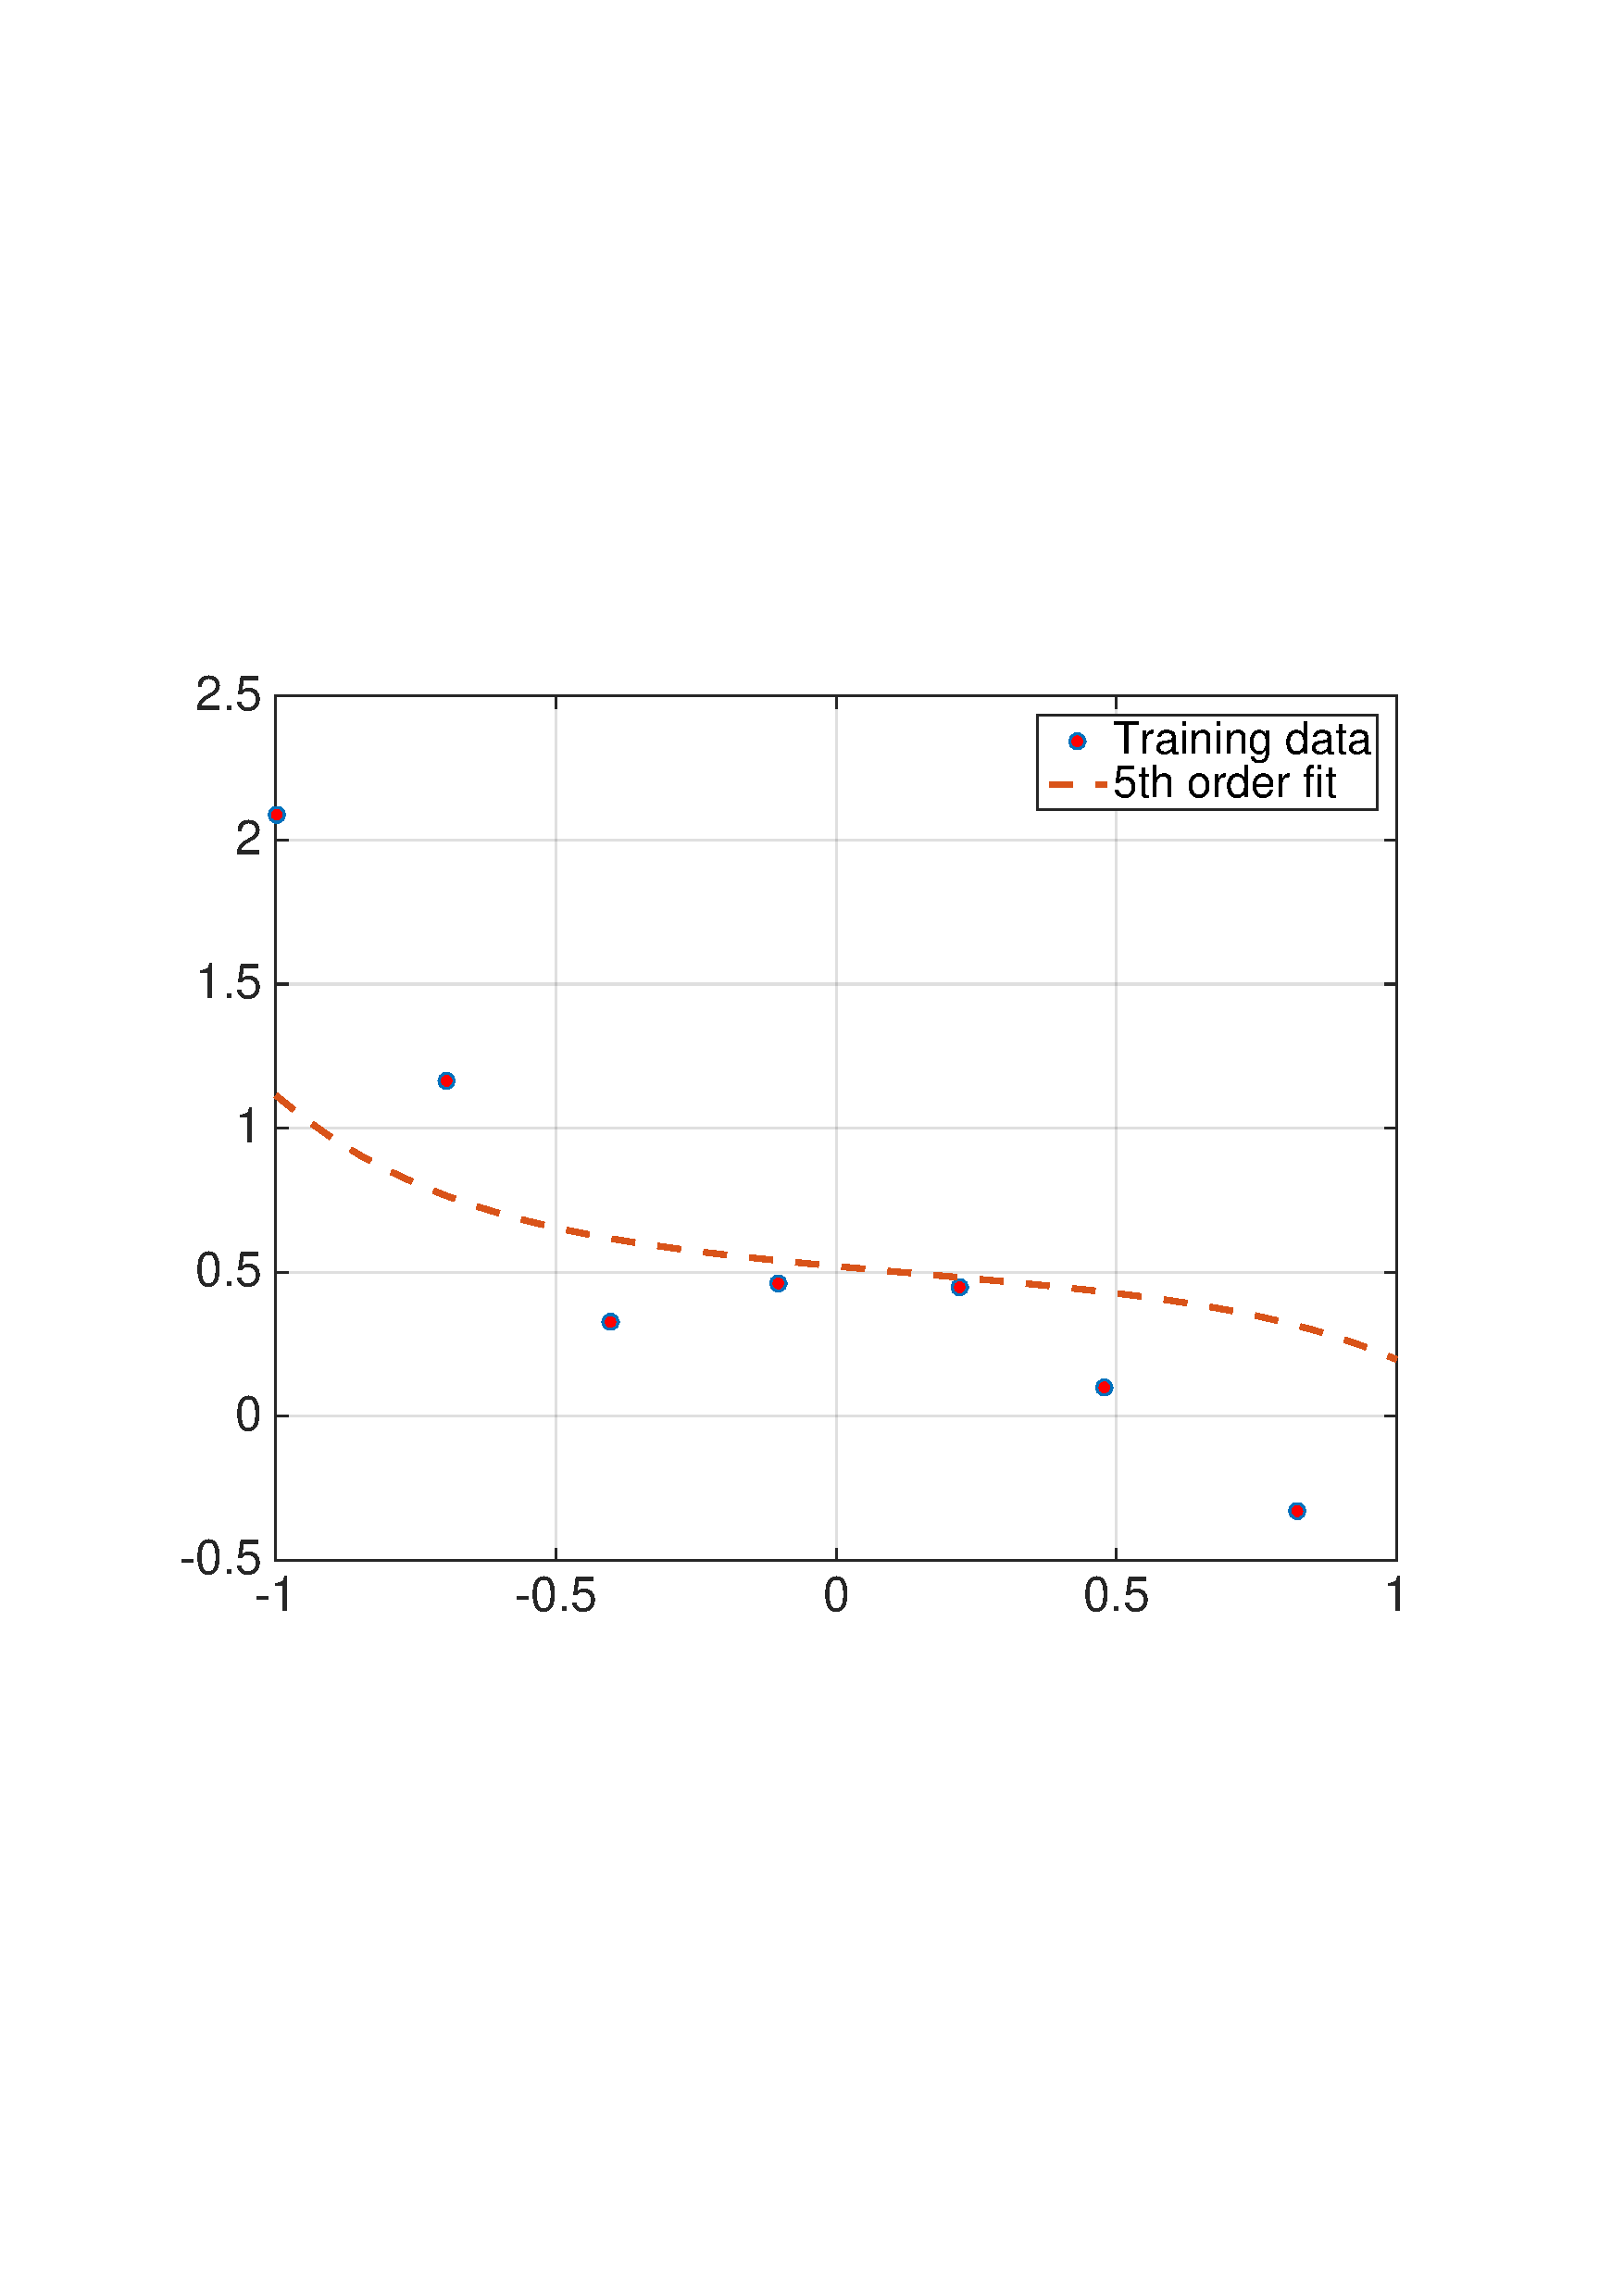
\includegraphics[width=.32\columnwidth]{lambda10}}
       \parbox{.32\columnwidth}{\center\scriptsize(a) $\lambda=0$}
       \parbox{.32\columnwidth}{\center\scriptsize(b) $\lambda=1$}
       \parbox{.32\columnwidth}{\center\scriptsize(c) $\lambda=10$}
       \caption{Regularized linear regression under different regularization parameters.}
       \label{fig:data}
       \end{center}
    \end{figure}

  We also give each element of $\theta$ under different settings of $\lambda$ in Table~\ref{tab:theta} Lager $\lambda$ exerts stronger penalties to the parameters (of the hypothesis function), especially the larger ones. Therefore, we have the norm of $\theta$ decreased with increasing $\lambda$.


    \begin{table}[htb]
    \caption{$\theta$ under different regularization parameters}
    \begin{center}
     \begin{tabular}{|c|c|c|c|} \hline
                    & $\lambda=0$ & $\lambda=1$ & $\lambda=10$ \\ \hline
       $\theta_0$   & 0.4725 & 0.3976 & 0.5205 \\ \hline
       $\theta_1$   & 0.6814 & -0.4207 & -0.1825 \\ \hline
       $\theta_2$   & -1.3801 & 0.1296 & 0.0606 \\ \hline
       $\theta_3$   & -5.9780 & -0.3975 & -0.1482 \\ \hline
       $\theta_4$   & 2.4418 & 0.1753 & 0.0743 \\ \hline
       $\theta_5$   & 4.7374 & -0.3394 & -0.1280 \\ \hline
       $\|\theta\|$ & 8.1690 & 0.8098 & 0.5931 \\ \hline
     \end{tabular}
    \end{center}
    \label{tab:theta}
    \end{table}


\section{Newton's Method for Regularized Logistic Regression}
%
  We apply Newton's method to non-linear regularized logistic regression with different $\lambda$'s. The results are visualized in Fig.~\ref{fig:log}. When $\lambda=0$ (such that we have a non-regularized logistic regression), the positive and negative training data are separated accurately by the resulting decision boundary. There is even an island negative region inside the positive region. Similar to the above case of regularized linear regression, the decision boundary is too precise to reflect the general trend of the training data. In another word, the decision boundary over-fits the training data in this case. The $\lambda = 1$ plot shows an simpler decision boundary which still separates the positives and negatives fairly well. On the other hand, $\lambda = 10$ is probably too high of a regularization parameter, as the boundary decision does not follow the data so well on in the lower-left region.
  %
  \begin{figure}[htb!]
       \begin{center}
       \parbox{.32\columnwidth}{\center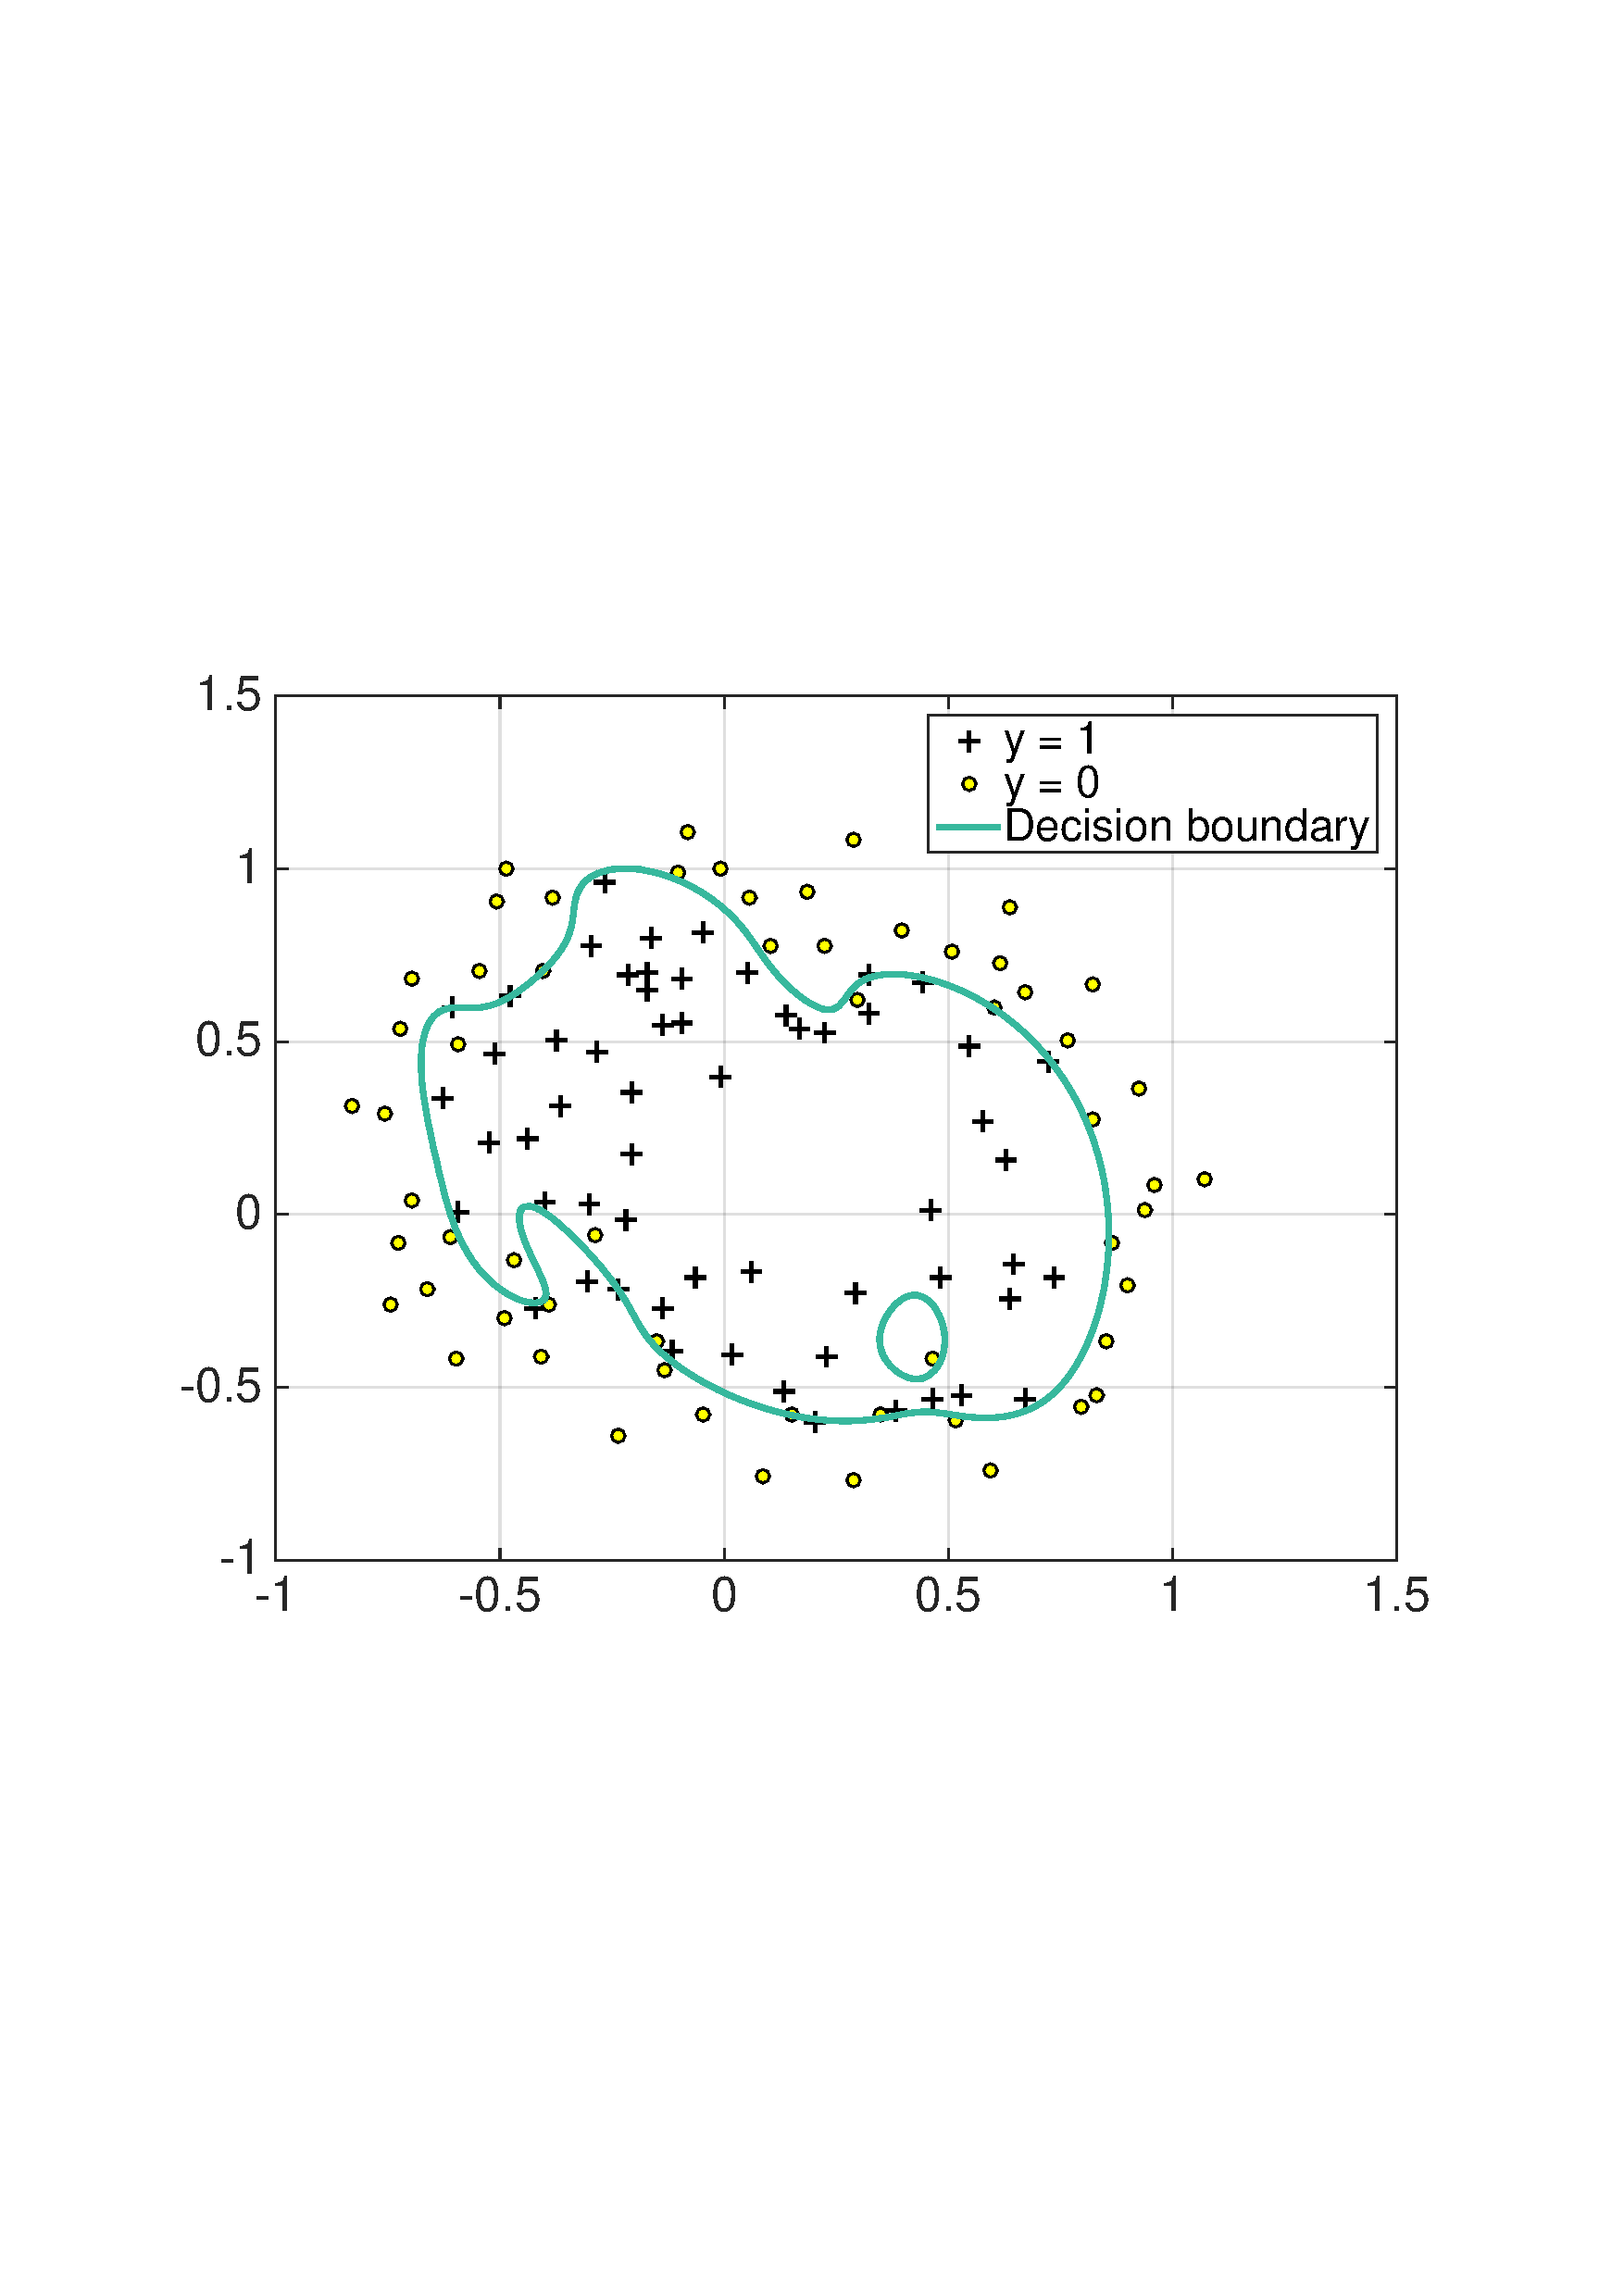
\includegraphics[width=.32\columnwidth]{exlambda0}}
       \parbox{.32\columnwidth}{\center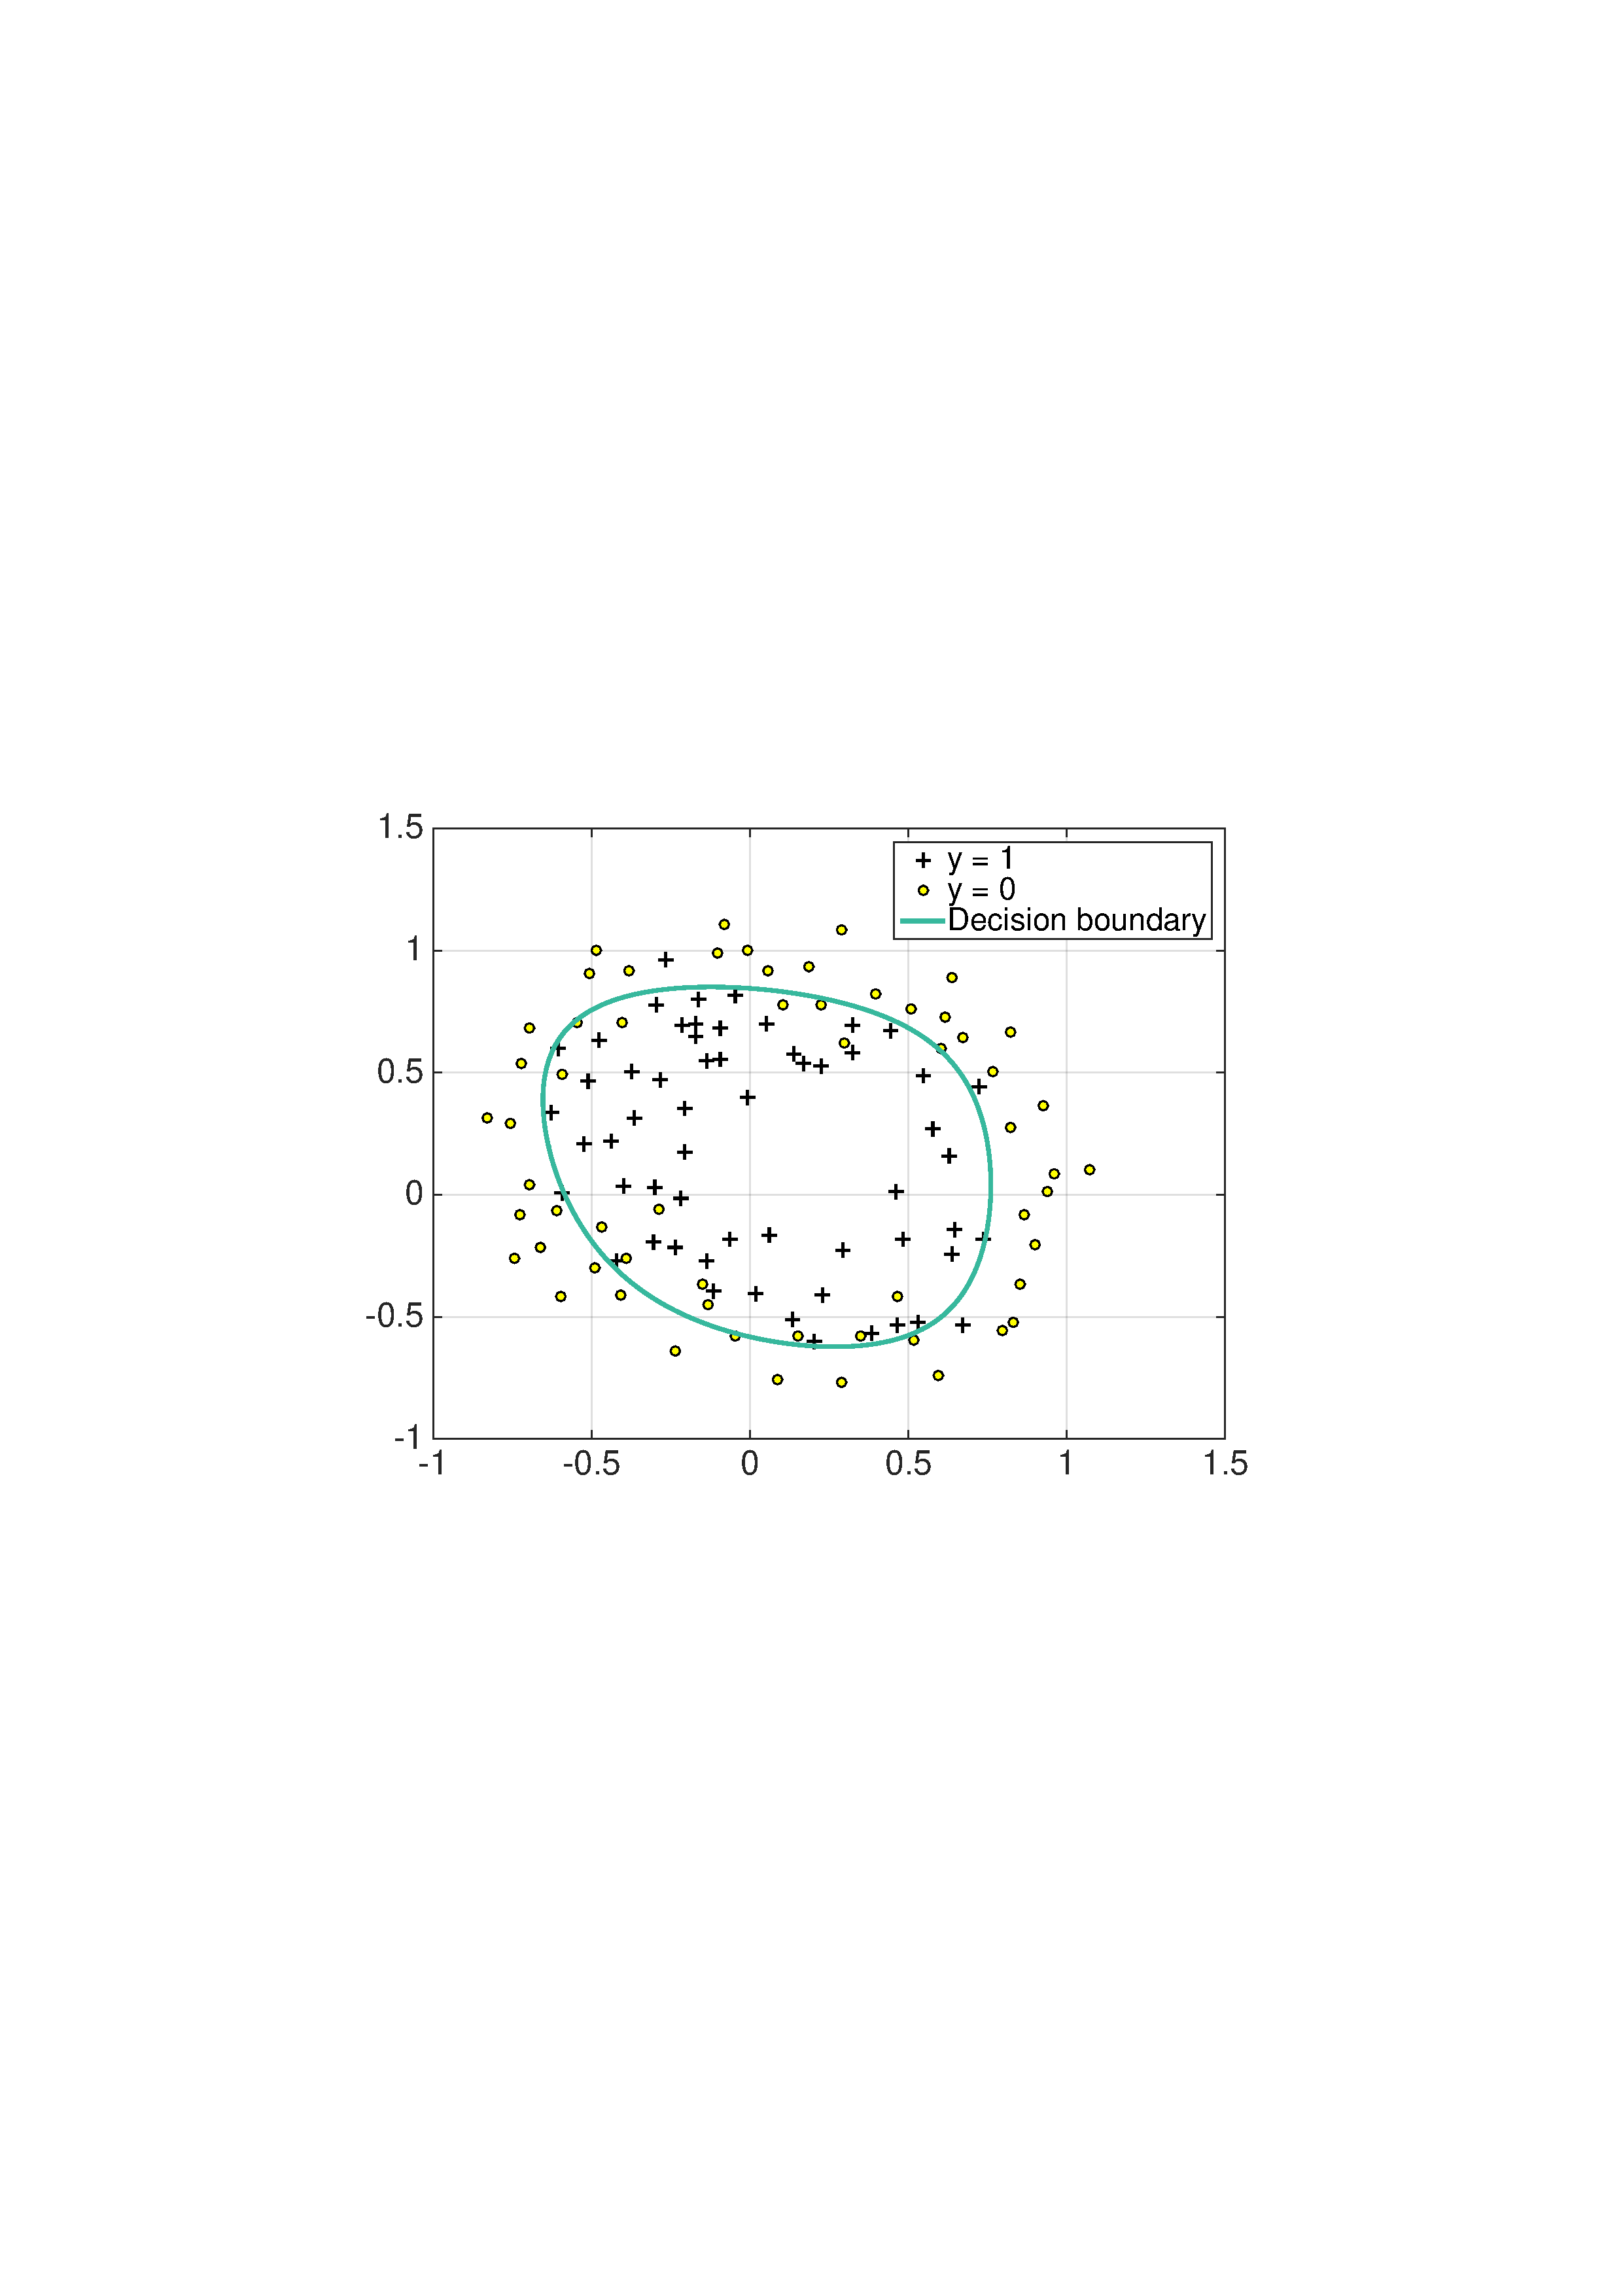
\includegraphics[width=.32\columnwidth]{exlambda1}}
       \parbox{.32\columnwidth}{\center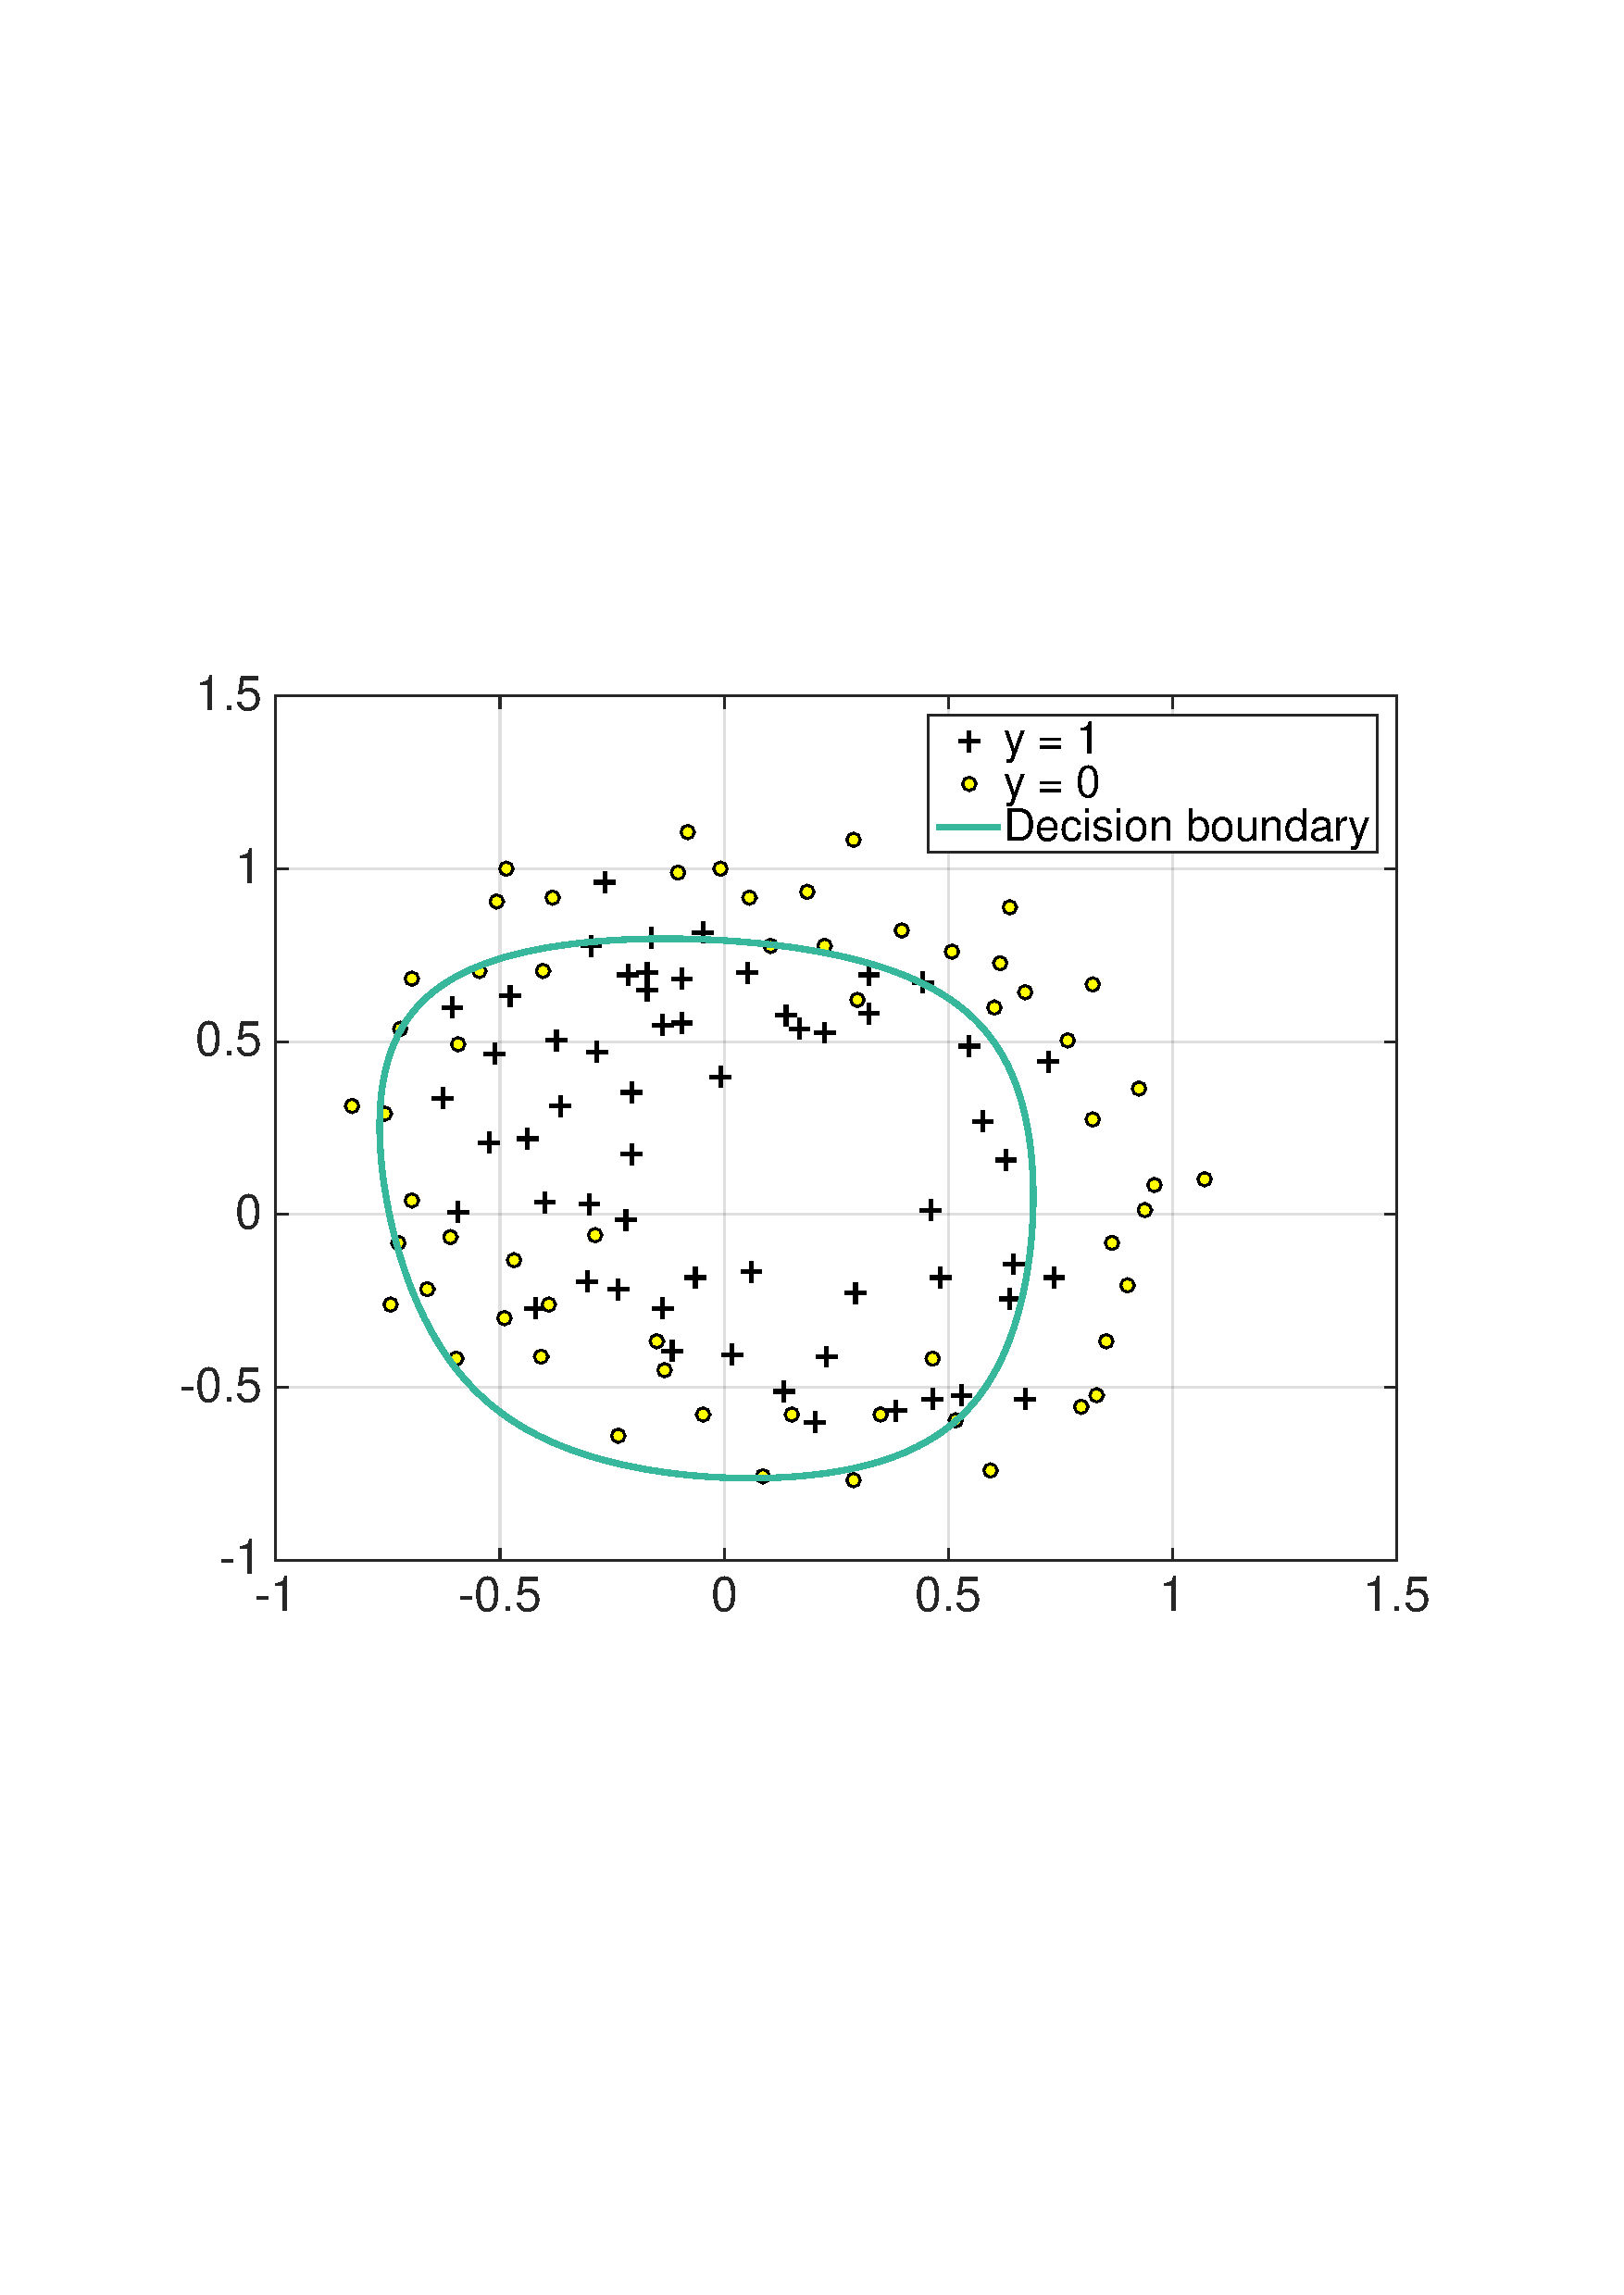
\includegraphics[width=.32\columnwidth]{exlambda10}}
       \parbox{.32\columnwidth}{\center\scriptsize(a) $\lambda=0$}
       \parbox{.32\columnwidth}{\center\scriptsize(b) $\lambda=1$}
       \parbox{.32\columnwidth}{\center\scriptsize(c) $\lambda=10$}
       \caption{Regularized logistic regression under different regularization parameters.}
       \label{fig:log}
       \end{center}
  \end{figure}

  We also report the norms of $\theta$'s under different $\lambda$'s in Table~\ref{tab:norm}. The norms of $\theta$ decrease as $\lambda$ increases. There are also visible fitting changes in the corresponding plots.


  %
    \begin{table}[htb]
    \caption{$\theta$ under different regularization parameters}
    \begin{center}
     \begin{tabular}{|c|c|c|c|} \hline
                    & $\lambda=0$ & $\lambda=1$ & $\lambda=10$ \\ \hline
       $\|\theta\|$ & $7.173\times 10^3$ & $4.240$ & $0.9384$ \\ \hline
     \end{tabular}
    \end{center}
    \label{tab:norm}
    \end{table}

\end{document}








  \end{lstlisting}
  %


